%%
%% Copyright 2025 Oxford University Press
%%
%% This file is part of the 'oup-authoring-template Bundle'.
%%
%% It may be distributed under the conditions of the LaTeX Project Public
%% License, either version 1.3 of this license or (at your option) any
%% later version.
%%

\documentclass[unnumsec,webpdf,modern,large]{oup-authoring-template}

\graphicspath{{Fig/}}

\makeatletter
\providecommand{\city}[1]{#1}
\makeatother

\begin{document}

\journaltitle{Nucleic Acids Research}
\DOI{00.0000/nar/XXXX}
\copyrightyear{2026}
\pubyear{2026}
\access{Advance Access Publication Date: Day Month Year}
\appnotes{Database Issue}
\makeatletter
\def\ps@opening{%
  \def\@oddhead{\raisebox{-40pt}[0pt][0pt]{\hbox to \textwidth{%
    {\vbox to 19mm{\hbox{}\vfill\hbox to 122mm{{%
    \parbox{290pt}{\raggedright{{\sffamily\fontsize{6.5bp}{9.5bp}\selectfont\textit{\@journaltitle},\ \@copyrightyear, \@volume,  \thepage--\thelastpage\par\vskip0pt}}
    {\sffamily\fontsize{6.5bp}{9.bp}\selectfont\@DOI\par%
    \ifx\@access\@empty\else\@access\par\fi\vskip0pt
    \ifx\@specialissue\@empty\else\@specialissue\par\fi
    \ifx\@appnotes\@empty\else\sffamily\fontsize{7bp}{9.bp}\textbf{\@appnotes}\par\fi
    }
      }}%
    }\vfill\hbox{}}}\hfill\smash{
\includegraphics[height=60pt]{NAR.png}}}}}%}\vfill\hbox{}}}\hfill\smash{
\includegraphics[height=80pt]{NAR.png}}}}}%
  \def\@evenhead{\@oddhead}%
  \def\@oddfoot{\parbox{\textwidth}{%
    \textcolor{black!60}{\rule{\textwidth}{.5pt}}\par\vspace*{5pt}\fontsize{6.25bp}{8bp}\selectfont\@history\par\raggedright
    \fontseries{m}\selectfont$\copyright$ The Author(s) \@pubyear. Copyright and licence statements to be updated by the publisher during production.
  }}%
  \def\@evenfoot{\@oddfoot}%
}
\makeatother\firstpage{1}

\title[PETadex]{PETadex: a comprehensive database of plastic-degrading enzyme sequence diversity}

\author[1,$\ast$]{Dennis Zhu}
\author[1]{Thomas Quigley}
\author[1]{Wisam Al Abed}
\author[1]{Artem Babaian}

\address[1]{\orgdiv{Donnelly Centre for Cellular and Biomolecular Research}, \orgname{University of Toronto}, \orgaddress{\city{Toronto}, \state{ON}, \country{Canada}}}

\corresp[$\ast$]{Corresponding author. \href{mailto:artem.babaian@utoronto.ca}{artem.babaian@utoronto.ca}}

\received{Date}{0}{Year}
\revised{Date}{0}{Year}
\accepted{Date}{0}{Year}

\abstract{Polyethylene terephthalate (PET) is among the most abundant synthetic pollutants in the environment, and enzymatic degradation by PET hydrolases (PETases) represents a promising route toward biological plastic remediation. Despite growing interest in PETase engineering and discovery, existing databases capture only a small fraction of the predicted PETase-like sequence diversity present in metagenomic and environmental sequencing data. While existing curated databases capture hundreds of experimentally verified enzymes, they represent only a narrow piece of the PETase sequence landscape; the vast majority of PETase-like diversity encoded in environmental and metagenomic data remains uncatalogued and inaccessible. Addressing this, a comprehensive database and web platform cataloguing 216.7 million PETase-like protein sequences drawn from the Logan database and organized into approximately 65,000 families via a three-level clustering hierarchy. PETadex integrates functional annotations (InterProScan domain assignments on family centroids, SignalP signal peptide predictions), NCBI metadata enrichment for 1.2 million non-redundant variant sequences to date (of an estimated 2.7 million total), and 259 standardized activity measurements from a unified BHET hydrolysis assay. The platform provides a serverless MMseqs2-based sequence search, an interactive ESM-2 embedding landscape (Atlas) for navigating enzyme family relationships, and a suite of visualization tools including beeswarm plots and functional annotation dot plots. Applying this landscape revealed families containing multi-domain (cocktail enzyme) architectures that sequence-identity clustering alone does not resolve, and cross-referencing with environmental metadata suggests a subset of these map to sulfur-rich, aerobic environments. PETadex is freely available at https://petadex.net.}

\keywords{PETase, plastic degradation, metagenomics, enzyme database, protein language model, sequence search}

\maketitle

\begin{figure*}[b]
\centering
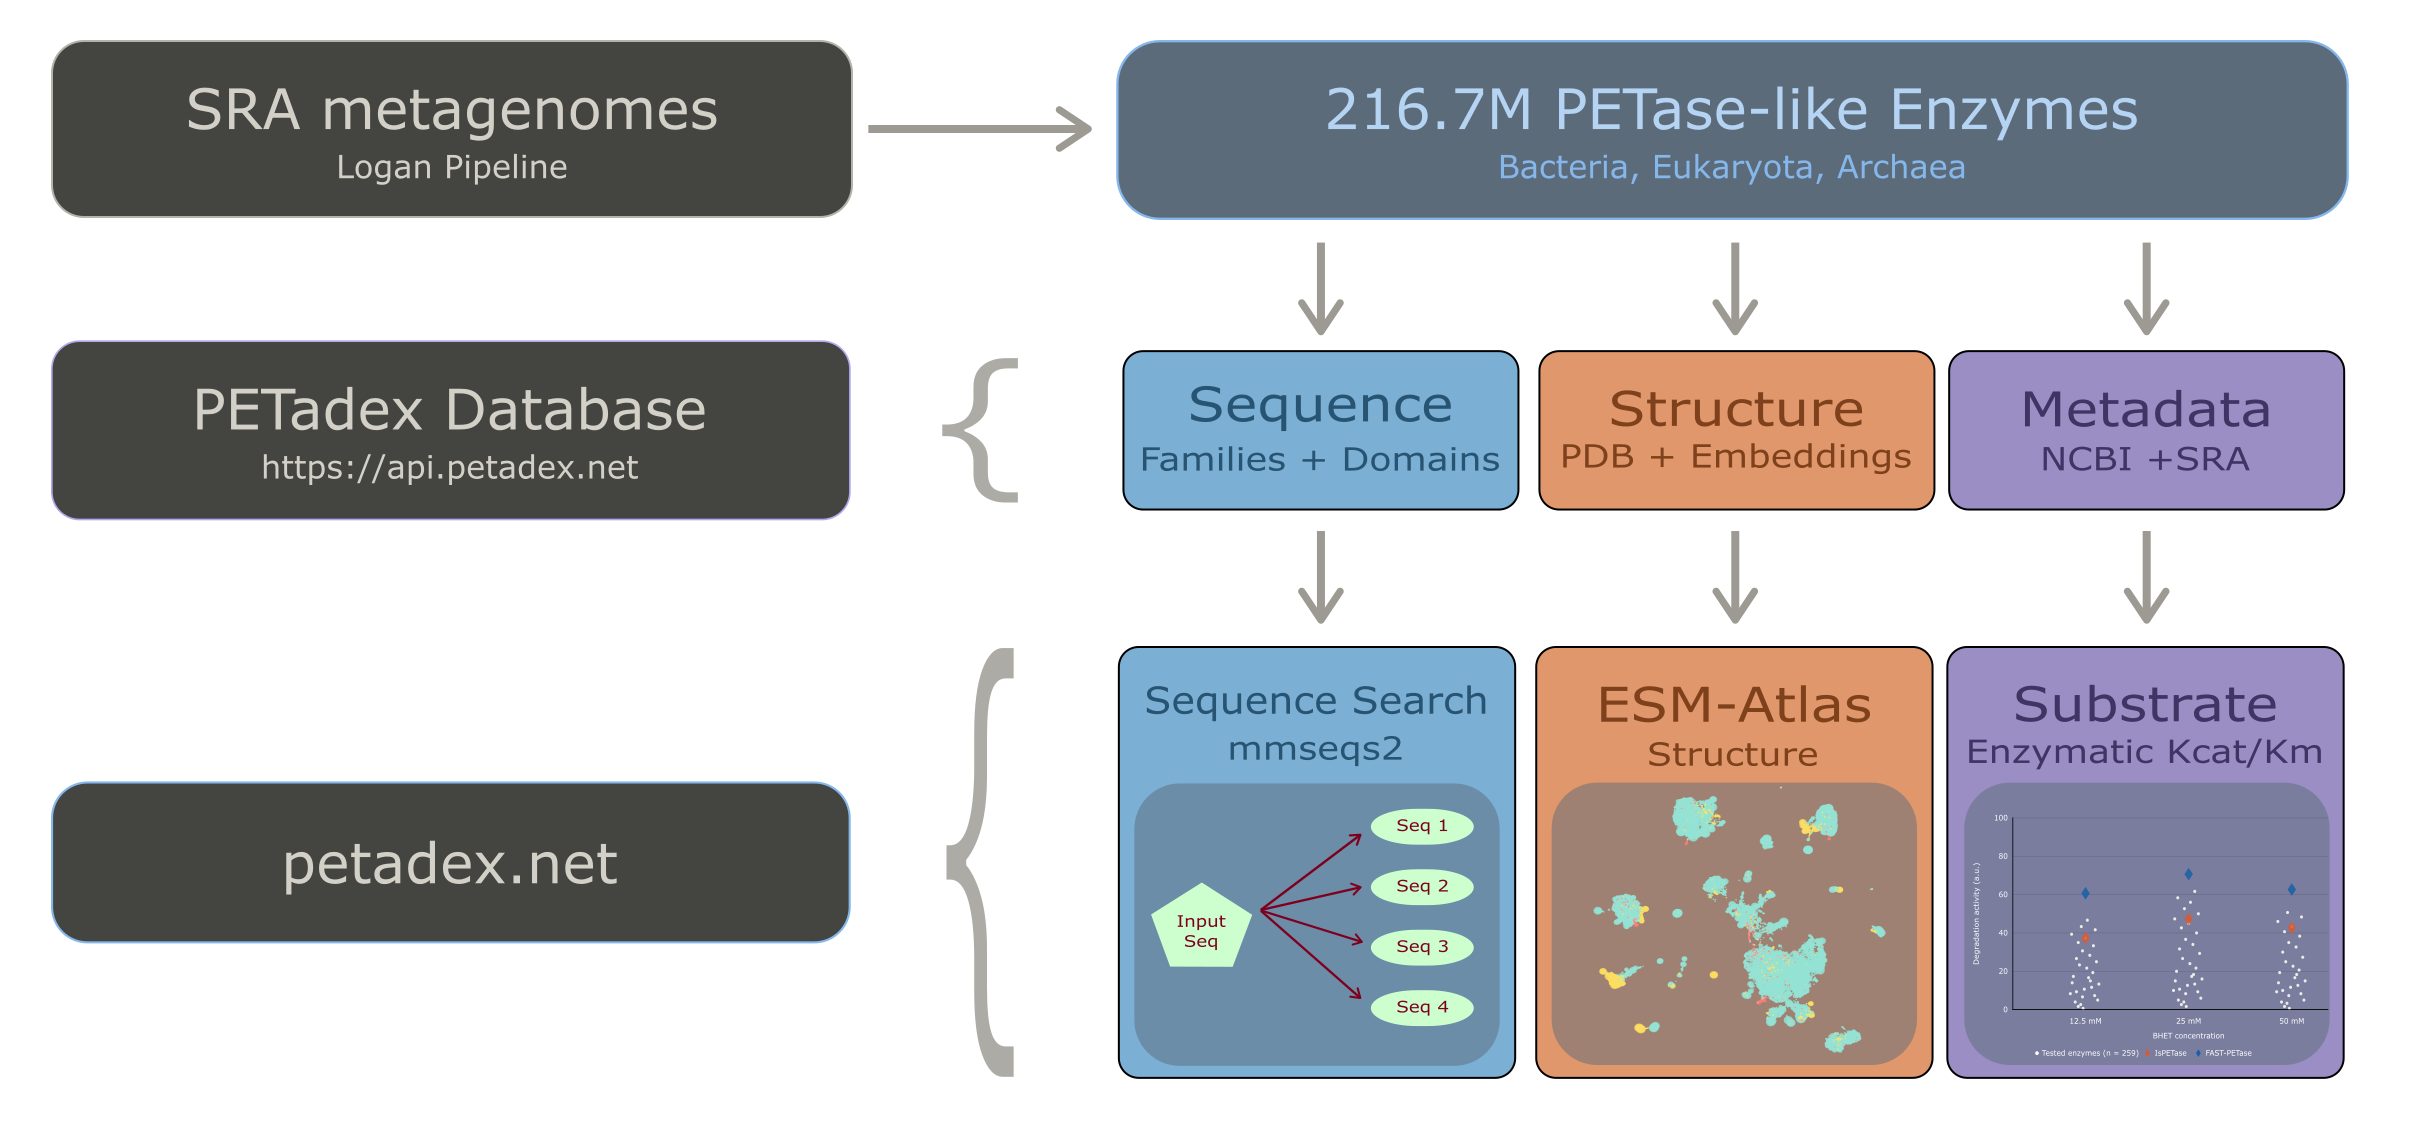
\includegraphics[width=\textwidth]{petadex_graphical_abstract.png}
\caption*{Graphical Abstract}
\end{figure*}

%\saythanks

%% ============================================================
\section{Introduction}

Plastic pollution is a defining environmental challenge of the 21st century. Global plastic production exceeded 400 million tonnes in 2022, and polyethylene terephthalate (PET) accounts for a substantial fraction of this output, driven primarily by beverage bottle and textile fiber manufacturing \citep{geyer_production_2017,noauthor_plastics_nodate}. PET is highly resistant to natural degradation, persisting in the environment for centuries and accumulating across marine, freshwater, and terrestrial ecosystems \citep{chamas_degradation_2020}. The resulting ecological and public health consequences have motivated an urgent search for sustainable remediation strategies, among which biological degradation by microbial enzymes has emerged as a particularly promising approach \citep{wei_microbial_2017,tournier_engineered_2020}.

The landmark discovery of the bacterium \textit{Ideonella sakaiensis} and its PET-degrading enzyme (IsPETase) in 2016 demonstrated that nature has already evolved enzymatic machinery capable of depolymerizing PET under mild conditions \citep{yoshida_bacterium_2016}. Since then, a growing number of PET hydrolases have been identified and characterized from diverse microbial taxa, including cutinases, lipases, and esterases that exhibit varying degrees of PET-degrading activity \citep{danso_plastics_2019,kawai_current_2019}. Engineering efforts have produced thermostable and catalytically enhanced variants with potential industrial applications, most notably the FAST-PETase and LCC variants \citep{lu_machine_2022,tournier_engineered_2020}. These advances have established enzymatic PET degradation as a viable component of circular plastic economy strategies.

Despite this progress, the resources available for exploring PETase sequence diversity remain limited in scope. The PAZy database provides a curated catalogue of approximately 218 experimentally verified wild-type plastic-degrading enzymes, serving as the gold standard for literature-validated PETase data \citep{buchholz_plastics_2022}. PlasticDB links 329 proteins and 875 species to plastic degradation with associated metadata \citep{gambarini_plasticdb_2022}. While both resources are valuable for their curation depth, they operate at a fundamentally different scale from the vast sequence diversity recoverable from modern metagenomic datasets. The explosion of environmental sequencing through initiatives such as the Sequence Read Archive (SRA) has generated petabases of data in which millions of uncharacterized PETase-like sequences are likely embedded, yet no existing platform provides systematic access to this diversity \citep{leinonen_sequence_2011}.

To address this gap, we developed PETadex (PET-active enzyme index), a database and web platform that catalogues 216.7 million PETase-like protein sequences derived from large-scale mining of metagenomic and environmental sequencing data. Building on the petaSearch pipeline and sequence discovery work described in Logan \textit{et al.}\ \citep{chikhi_logan_2025}, PETadex organizes this sequence space into approximately 65,000 families through a three-level clustering hierarchy and enriches it with functional annotations, NCBI metadata, and standardized experimental activity data. The platform provides a serverless sequence search, an interactive ESM-2 embedding landscape for family-level exploration, and a suite of tools designed to make the full breadth of predicted PETase diversity navigable and discoverable by the research community.

%% ============================================================
\section{Materials and Methods}

\subsection{Data sources and sequence acquisition}

The PETadex sequence corpus originates from the large-scale mining of the NCBI Sequence Read Archive (SRA) performed using the Serratus platform \citep{edgar_petabase-scale_2022} and the petaSearch pipeline, as described in Logan \textit{et al.}\ \citep{chikhi_logan_2025}. Briefly, petaSearch applied translated nucleotide search against PETase profile hidden Markov models across the entirety of the publicly available SRA, identifying open reading frames with significant similarity to known PET hydrolases. This yielded a raw set of 216.7 million PETase-like protein sequences spanning diverse microbial taxa and environmental contexts. Sequences were subsequently clustered at multiple identity thresholds using MMseqs2 \citep{steinegger_mmseqs2_2017} to produce a three-level hierarchy: components (broad groupings at low identity), families (intermediate clusters, approximately 65,000 total), and centroids (representative sequences for each family). A non-redundant variant dictionary of approximately 2.7 million sequences links individual accessions to their corresponding family centroids, providing the bridge between raw sequence diversity and the curated family-level annotations described below.

\subsection{Functional annotation}

Functional domain annotations were computed for all family centroids (approximately 65,000 sequences) using InterProScan 5 \citep{jones_interproscan_2014}, assigning Pfam, Gene3D, SUPERFAMILY, and other member database annotations to each representative sequence. Signal peptide predictions were generated using SignalP 6.0 \citep{teufel_signalp_2022} on the same centroid set. These annotations are propagated to all members of a given family through the clustering hierarchy, enabling domain and signal peptide information to be displayed for any sequence in the database without requiring individual annotation of all 216.7 million entries. All annotations are surfaced directly in the web interface, allowing users to browse, filter, and explore domain architectures interactively rather than consulting static tables.

\subsection{NCBI metadata enrichment}

Functional domain annotations were computed for all family centroids (approximately 65,000 sequences) using InterProScan 5 \citep{jones_interproscan_2014}, assigning Pfam, Gene3D, SUPERFAMILY, and other member database annotations to each representative sequence. Signal peptide predictions were generated using SignalP 6.0 \citep{teufel_signalp_2022} on the same centroid set. These annotations are surfaced directly in the web interface to support general exploration of domain architectures across the database. Broadly, domain classifications derived from InterProScan are consistent with sequence identity-based clustering, though outliers exist and have been flagged for downstream analysis. Metadata including taxonomic origin, source organism, environmental sampling context, and NCBI accession information are propagated to all members of a given family through the clustering hierarchy, enabling rich contextual information to be displayed for any sequence in the database without requiring individual retrieval across all 216.7 million entries.

\subsection{Database architecture and web platform}

PETadex is deployed as a three-tier web application (Figure~\ref{fig:architecture}). The frontend is a static site built with Gatsby \citep{noauthor_best_nodate} and hosted on GitHub Pages at \url{https://petadex.net}. User requests are routed through AWS API Gateway to a serverless Node.js/Express backend deployed on AWS Lambda via the Serverless Framework \citep{noauthor_serverless_nodate}. The backend queries a PostgreSQL database hosted on AWS RDS, which stores the core data entities: enzyme sequences, clustering taxonomy (component, family, centroid relationships), the variant dictionary, NCBI/SRA metadata, InterProScan annotations, SignalP predictions, experimental activity data, and precomputed UMAP atlas coordinates. Pre-computed materialized views in PostgreSQL enable responsive queries at scale, avoiding expensive joins at request time. Phylogenetic trees and other precomputed assets are stored in Amazon S3 for asynchronous retrieval by the client.

\begin{figure*}[!htbp]
\centering
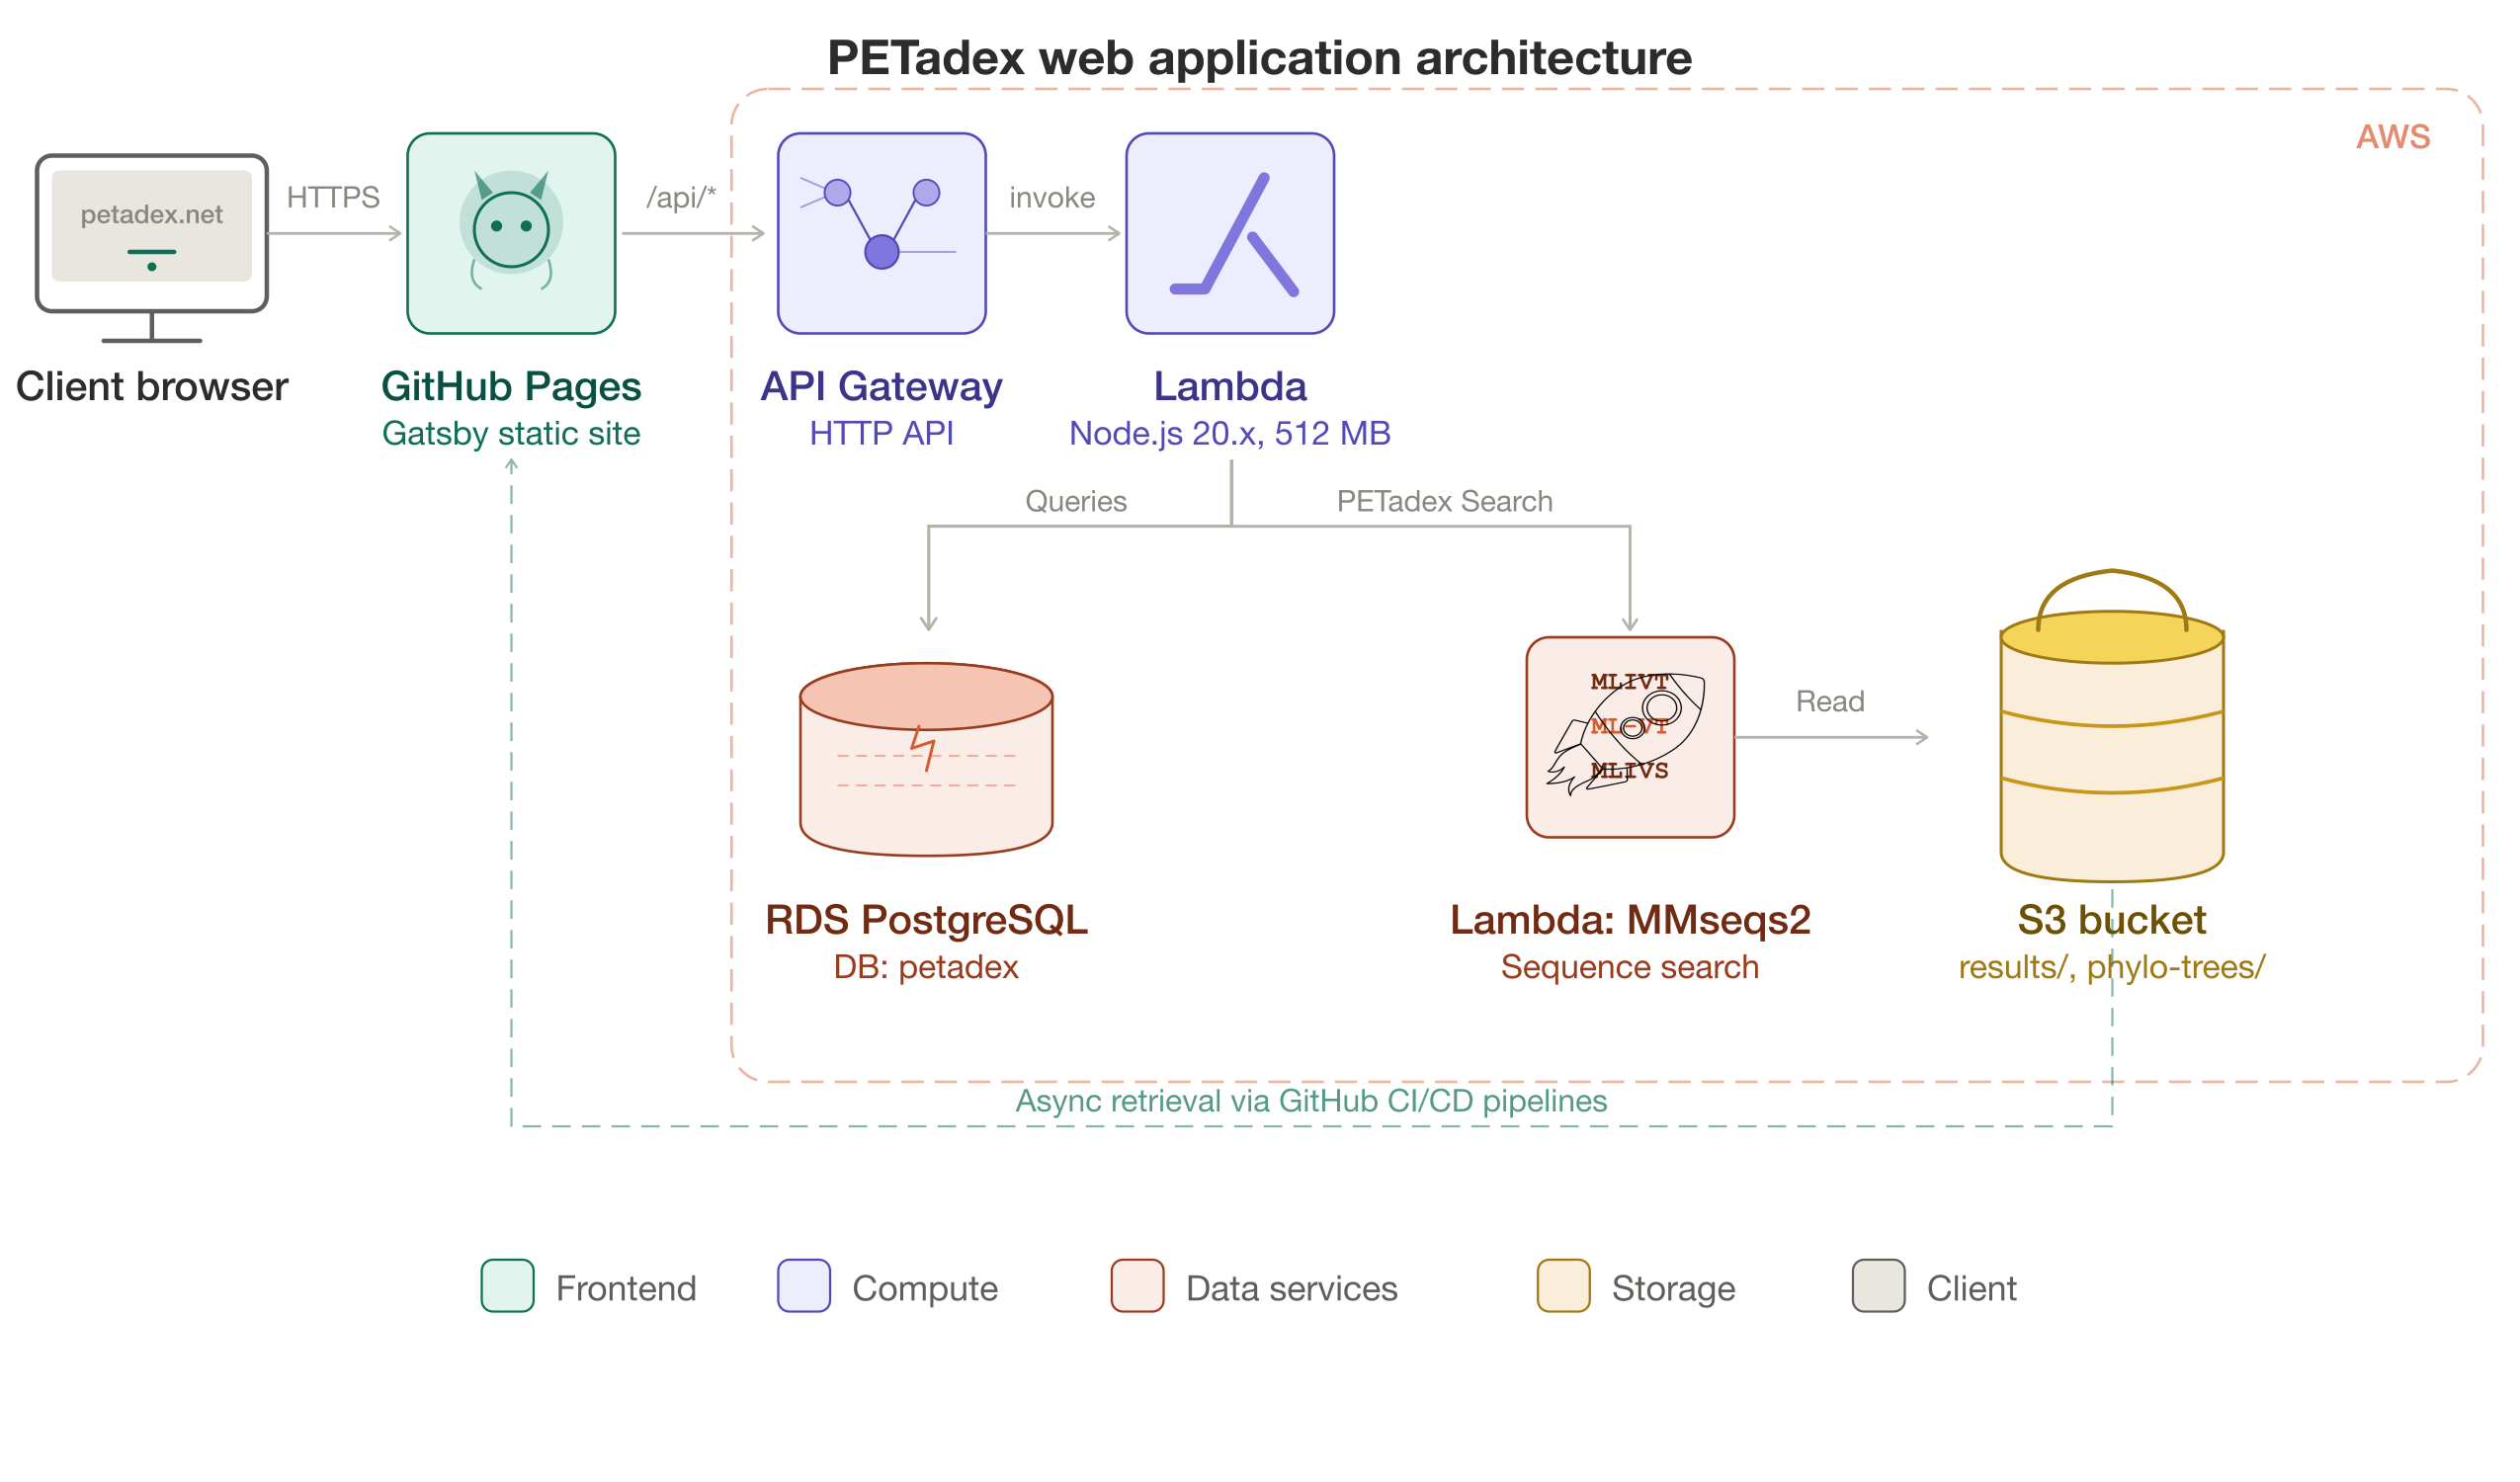
\includegraphics[width=\textwidth]{petadex_architecture.png}
\caption{\textbf{Architecture of the PETadex web platform.} User requests are served by a Gatsby static site hosted on GitHub Pages (petadex.net) and routed through AWS API Gateway to a serverless Node.js backend (AWS Lambda). The backend queries a PostgreSQL database (AWS RDS) for enzyme family metadata and invokes a dedicated Lambda function for MMseqs2 sequence similarity searches against the PETadex sequence corpus. Precomputed phylogenetic trees and search results are stored in Amazon S3 for asynchronous retrieval.}
\label{fig:architecture}
\end{figure*}

\subsection{Sequence search}

PETadex provides protein sequence search powered by MMseqs2 \citep{steinegger_mmseqs2_2017}, executed via a dedicated AWS Lambda function. Users submit a FASTA-formatted protein sequence through the web interface with a configurable maximum number of results. The Lambda function runs MMseqs2 against the PETadex sequence database and returns, for each hit: accession, organism, percent identity, E-value, bit score, query coverage, alignment length, and query/target coordinate ranges. Results are further enriched with database-derived fields including family classification, component assignment, and phylogenetic tree availability. Identical queries are cached using deterministic deduplication to avoid redundant computation. Response metadata includes the database size, search execution time, and total number of hits returned.

\subsection{ESM-2 embedding landscape}

To provide a structure-aware view of PETase family relationships, ESM-2 protein language model embeddings \citep{lin_evolutionary-scale_2023} were computed for all family centroids (approximately 65,000 sequences). The high-dimensional embeddings were projected to two dimensions using UMAP \citep{mcinnes_umap_2020} to produce the Atlas view, an interactive visualization in which each point represents a PETadex family and spatial proximity reflects structural and functional similarity as captured by the language model. The Atlas is rendered as an interactive scatter plot in the web interface, allowing users to pan, zoom, select individual families, and cross-reference with metadata and annotation layers. This provides a complementary lens to the sequence-identity-based clustering: while MMseqs2 clusters capture local sequence similarity, the ESM-2 embeddings capture broader structural and functional relationships that may not be apparent from primary sequence alone.

\subsection{Substrate activity comparison}

Experimental plate-reader data for the BHET hydrolysis assay are served through a dedicated substrate comparison interface (\texttt{/substrate}). Raw data consist of per-gene, per-substrate median pixel intensity measurements at five timepoints (24, 48, 72, 96, and 120 h) across three BHET concentrations (12.5, 25, and 50 mM) (Figure~\ref{fig:substrate}). A degradation activity metric is computed server-side for each gene--substrate pair as the difference between the peak intensity value and the subsequent minimum intensity value across the timeseries. Four quality flags are assigned where applicable: \texttt{peak\_at\_end} (peak falls at the final timepoint; activity set to null), \texttt{peak\_at\_start} (peak at the first timepoint), \texttt{single\_degradation\_point} (only one timepoint separates peak from minimum), and \texttt{negative\_activity} (no degradation signal detected). These flags are surfaced in the web interface and included in downloaded data to allow users to apply their own quality thresholds.

%% ============================================================
\section{Results}

\subsection{Database scale and composition}

PETadex contains 216.7 million PETase-like protein sequences organized into approximately 65,000 families through the three-level clustering hierarchy described above. The non-redundant variant dictionary comprises 2.7 million sequences with NCBI metadata, representing the dereplicated diversity of the full corpus. Taxonomic analysis of the metadata-annotated fraction reveals that bacteria dominate the database (89.5\% of annotated sequences), followed by eukaryotes (8.6\%) and archaea (1.5\%), with viral and unclassified sequences comprising fewer than 0.1\% of entries (Figure~\ref{fig:metadata}A). The top source organisms are predominantly environmental and soil-associated lineages from the phyla Pseudomonadota, Chloroflexota, Actinomycetota, and Acidobacteriota (Figure~\ref{fig:metadata}B), reflecting the metagenomic origins of most sequences rather than well-characterized laboratory isolates. Family size follows a heavy-tailed distribution, with a small number of large families containing thousands of variants and a long tail of small families with fewer than ten members (Figure~\ref{fig:metadata}C). Temporal analysis of the 38.2\% of sequences with recorded collection dates shows a marked increase in PETase-like sequence deposition from 2015 onward, coinciding with the characterization of IsPETase by Yoshida \textit{et al.}\ \citep{yoshida_bacterium_2016} (Figure~\ref{fig:metadata}D). Metadata field completeness is high for core identifiers and taxonomy (over 99.7\%) but sparse for temporal and geographic annotations (Figure~\ref{fig:metadata}E).

\renewcommand{\topfraction}{0.9}
\renewcommand{\bottomfraction}{0.9}
\renewcommand{\textfraction}{0.1}
\renewcommand{\floatpagefraction}{0.8}
\renewcommand{\dbltopfraction}{0.9}
\renewcommand{\dblfloatpagefraction}{0.8}

\begin{figure*}[!htbp]
\centering
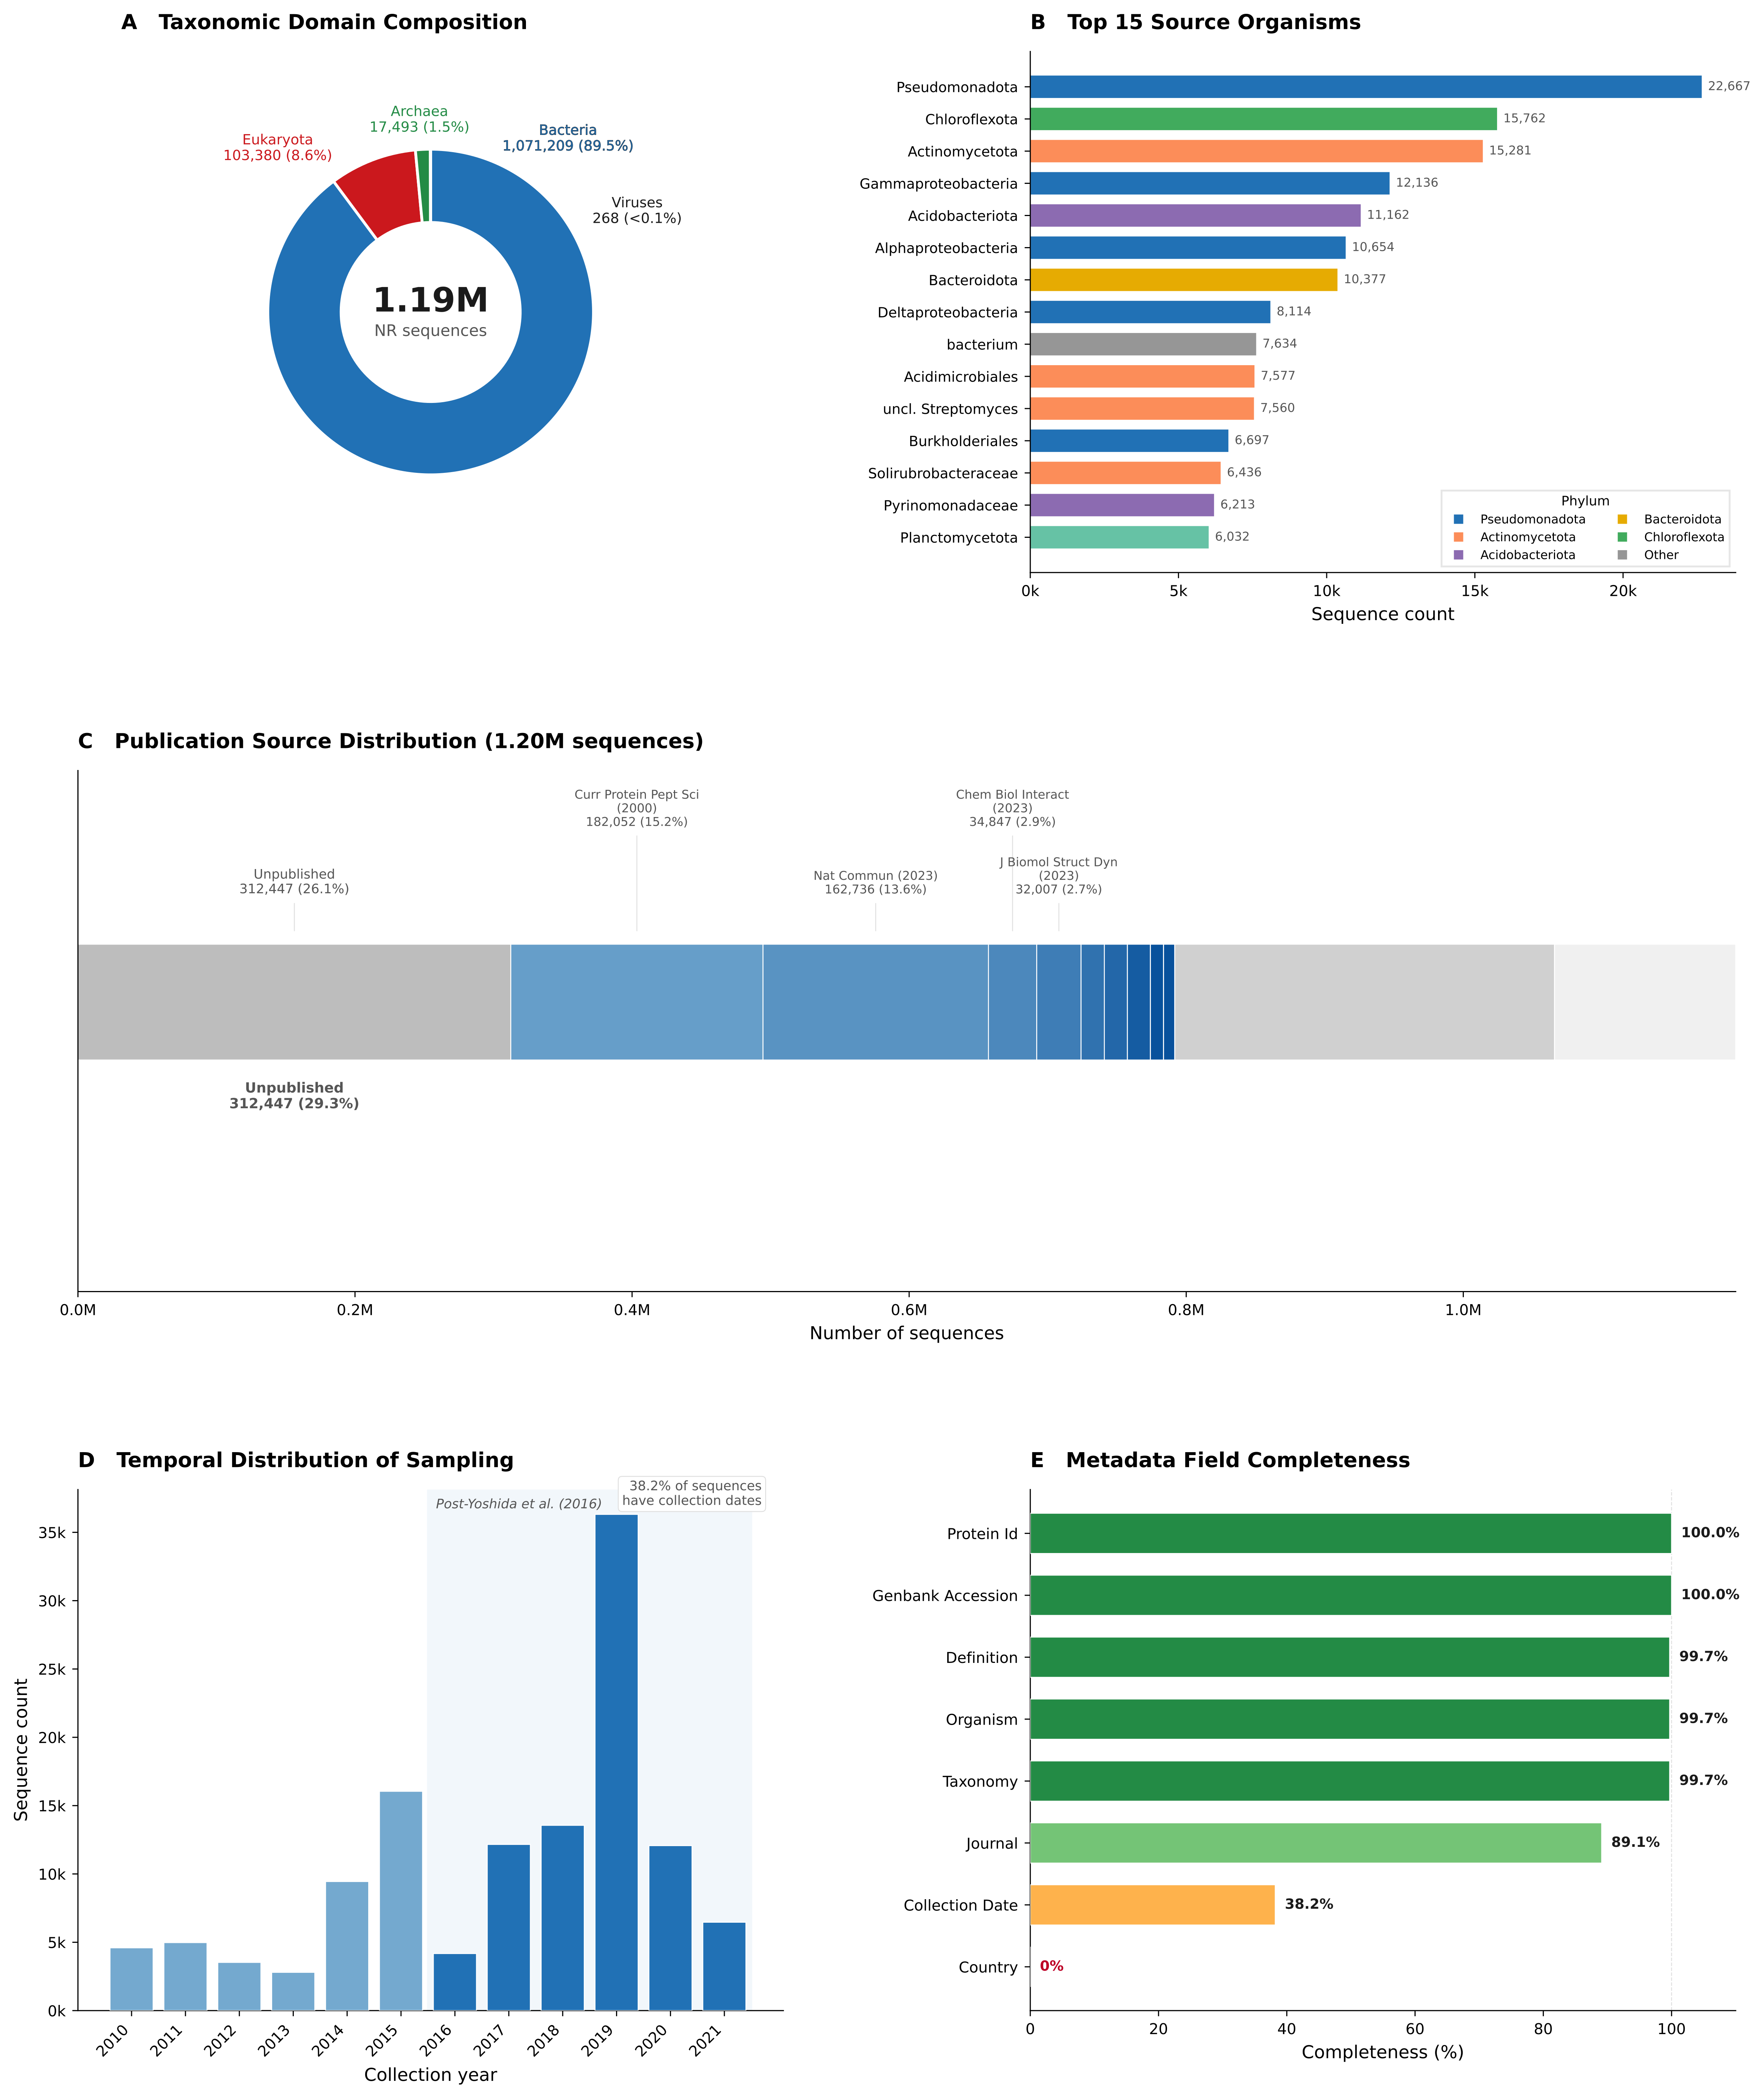
\includegraphics[width=0.75\textwidth]{petadex_metadata_figure.png}
\caption{\textbf{Metadata landscape of the PETadex non-redundant sequence database.} (A) Taxonomic domain composition of 1,196,644 annotated sequences, dominated by Bacteria (89.5\%) with representation across Eukaryota, Archaea, and Viruses. (B) Top 15 source organisms by sequence count, colored by phylum, revealing a predominance of environmental and soil-associated lineages. (C) Family size distribution across the database. (D) Temporal distribution of sample collection years (38.2\% of sequences annotated), showing increased deposition following the characterization of IsPETase \citep{yoshida_bacterium_2016}. (E) Metadata field completeness across all records.}
\label{fig:metadata}
\end{figure*}

The taxonomic composition of the database reflects the metagenomic origins of the underlying sequence data rather than a balanced sampling of PETase-producing organisms. The overwhelming dominance of Bacteria (89.5\%) is consistent with the fact that most environmental sequencing efforts target prokaryotic communities in soil, sediment, and aquatic habitats where PET debris accumulates. The representation of Eukaryota (8.6\%) and Archaea (1.5\%) suggests that PETase-like hydrolase domains are not restricted to bacterial lineages, though the extent to which these eukaryotic and archaeal sequences encode genuine PET-degrading activity remains largely untested. Among the top source organisms, the prevalence of lineages from Pseudomonadota, Chloroflexota, Actinomycetota, and Acidobacteriota points to a broad phylogenetic distribution of PETase-like sequences across environmentally abundant phyla, rather than concentration in a small number of specialist taxa.

The publication source distribution reveals that a substantial fraction of the database (29.3\%) derives from unpublished SRA submissions, while three large-scale metagenomic studies contribute over 45\% of the literature-linked entries. This concentration highlights both the power of a small number of large sequencing initiatives to shape the landscape of discoverable enzyme diversity and the potential for bias toward the environments and sampling strategies favored by those projects. The 10.9\% of sequences lacking any journal annotation represent an additional pool of uncharacterized data that may contain novel diversity but cannot currently be traced to a specific study context.

\begin{figure*}[!htbp]
\centering
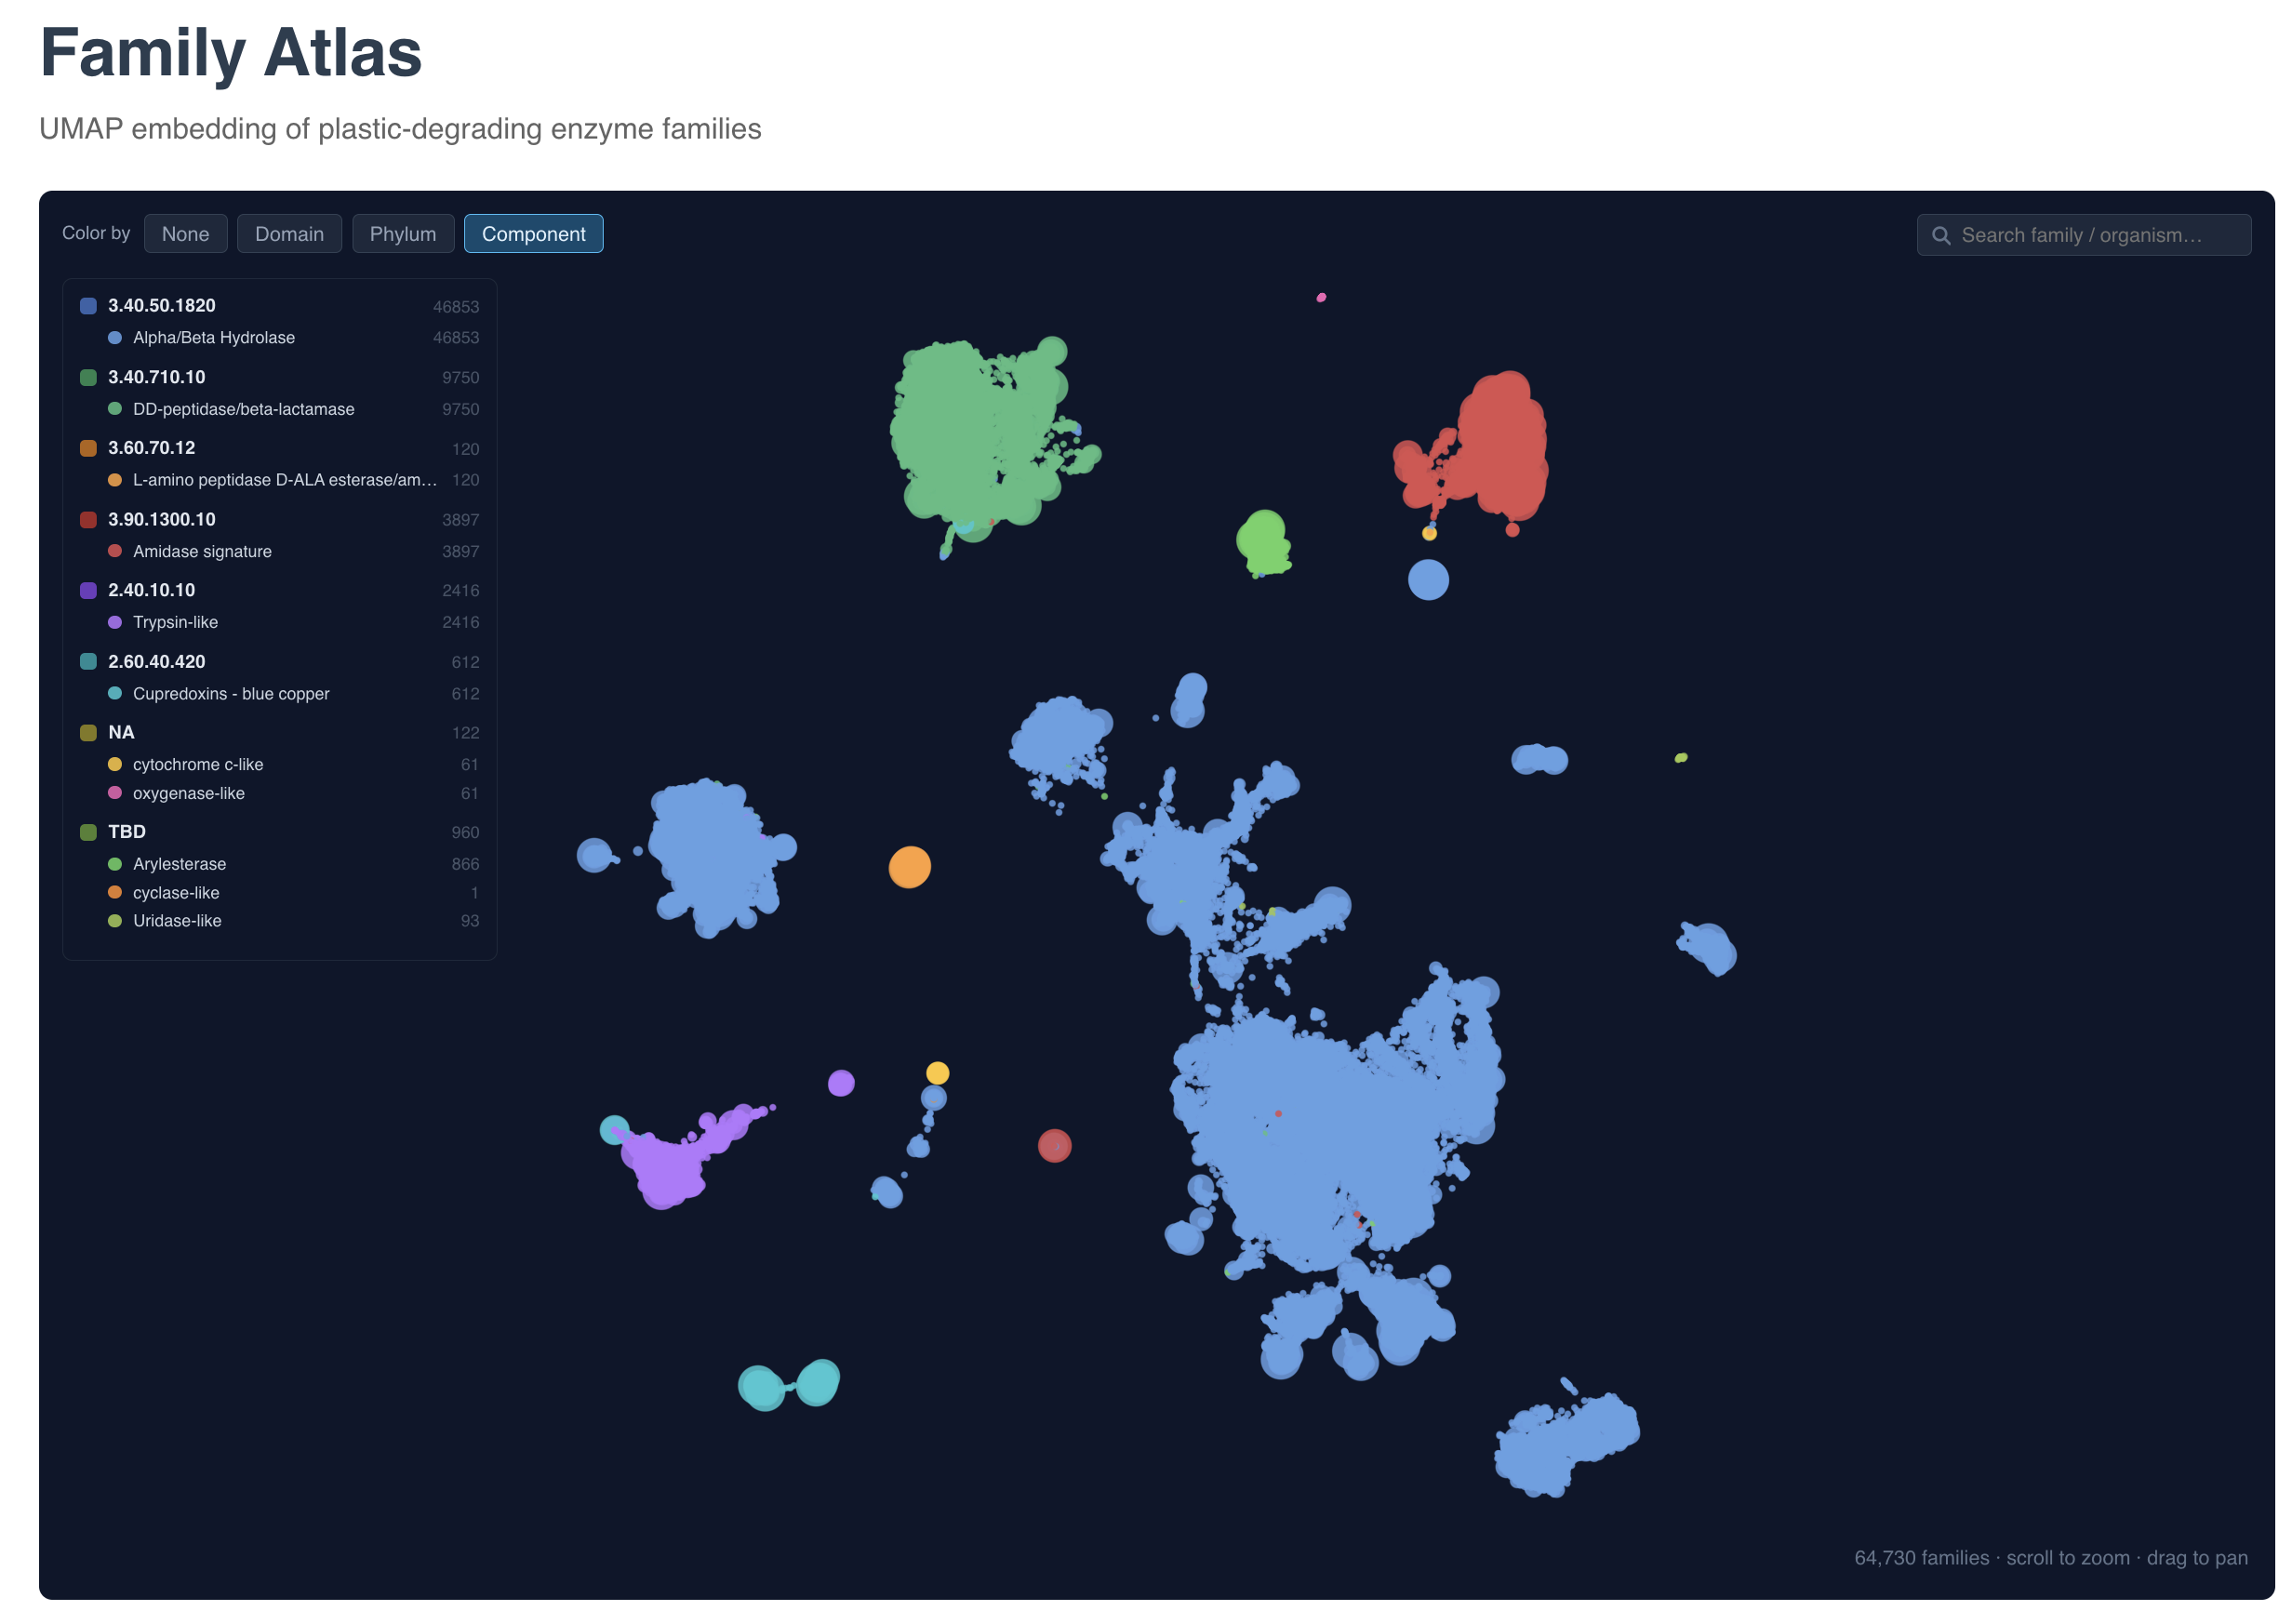
\includegraphics[width=\textwidth]{esm-landscape-transparent.png}
\caption{\textbf{ESM-2 embedding landscape (Atlas) of PETadex family centroids.} UMAP projection of ESM-2 embeddings computed for approximately 65,000 family centroids. Each point represents a PETadex family. The annotated region highlights a cluster of multi-domain (cocktail enzyme) families associated with sulfur-rich, aerobic environments, identified by cross-referencing embedding coordinates with NCBI environmental metadata. This cluster was not resolved by sequence-identity clustering alone.}
\label{fig:atlas}
\end{figure*}

The temporal distribution of collection dates, available for only 38.2\% of sequences, shows a clear inflection point around 2015, with deposition rates increasing sharply following the characterization of IsPETase by Yoshida \textit{et al.}\ \citep{yoshida_bacterium_2016} in 2016. This pattern likely reflects both increased research interest in PET-degrading enzymes and the broader expansion of environmental sequencing over the same period, making it difficult to attribute the trend to either factor alone. Metadata field completeness varies considerably across the database: core identifiers and taxonomic annotations are nearly complete (over 99.7\%), but temporal and geographic metadata remain sparse. Collection dates are recorded for 38.2\% of sequences, and country of origin is absent from all records in the current release. This gap in geographic metadata limits the ability to perform spatial analyses of PETase diversity and underscores the need for improved metadata standards in public sequence repositories.

\subsection{Visualization and exploration features}

PETadex provides several integrated visualization tools to support exploration of the sequence data. The ESM-2 Atlas (Figure~\ref{fig:atlas}) serves as the primary exploration interface, rendering the UMAP projection of all family centroids as an interactive landscape that users can navigate, zoom, and query. Search results from MMseqs2 queries are displayed as beeswarm plots that visualize the distribution of hits across percent identity, E-value, and other alignment statistics, enabling rapid assessment of the taxonomic and family diversity recovered by a given query. Functional annotation dot plots summarize InterProScan domain assignments across families or search result sets, providing an overview of domain architecture composition. Each enzyme entry page integrates sequence data, structural information (where available), domain annotations, signal peptide predictions, and experimental activity measurements into a unified view.

The substrate comparison page (\texttt{/substrate}) provides an interactive view of the BHET hydrolysis timeseries data across all three substrate concentrations (Figure~\ref{fig:substrate}). A scatter plot of per-gene activity values at two user-selected concentrations enables direct visual assessment of substrate preference, with benchmark enzymes (IsPETase, FAST-PETase) rendered as reference points. Users can toggle between raw intensity and computed activity metrics, filter by timepoint, and export the full timeseries or activity summary as CSV files.

\begin{figure*}[!htbp]
\centering
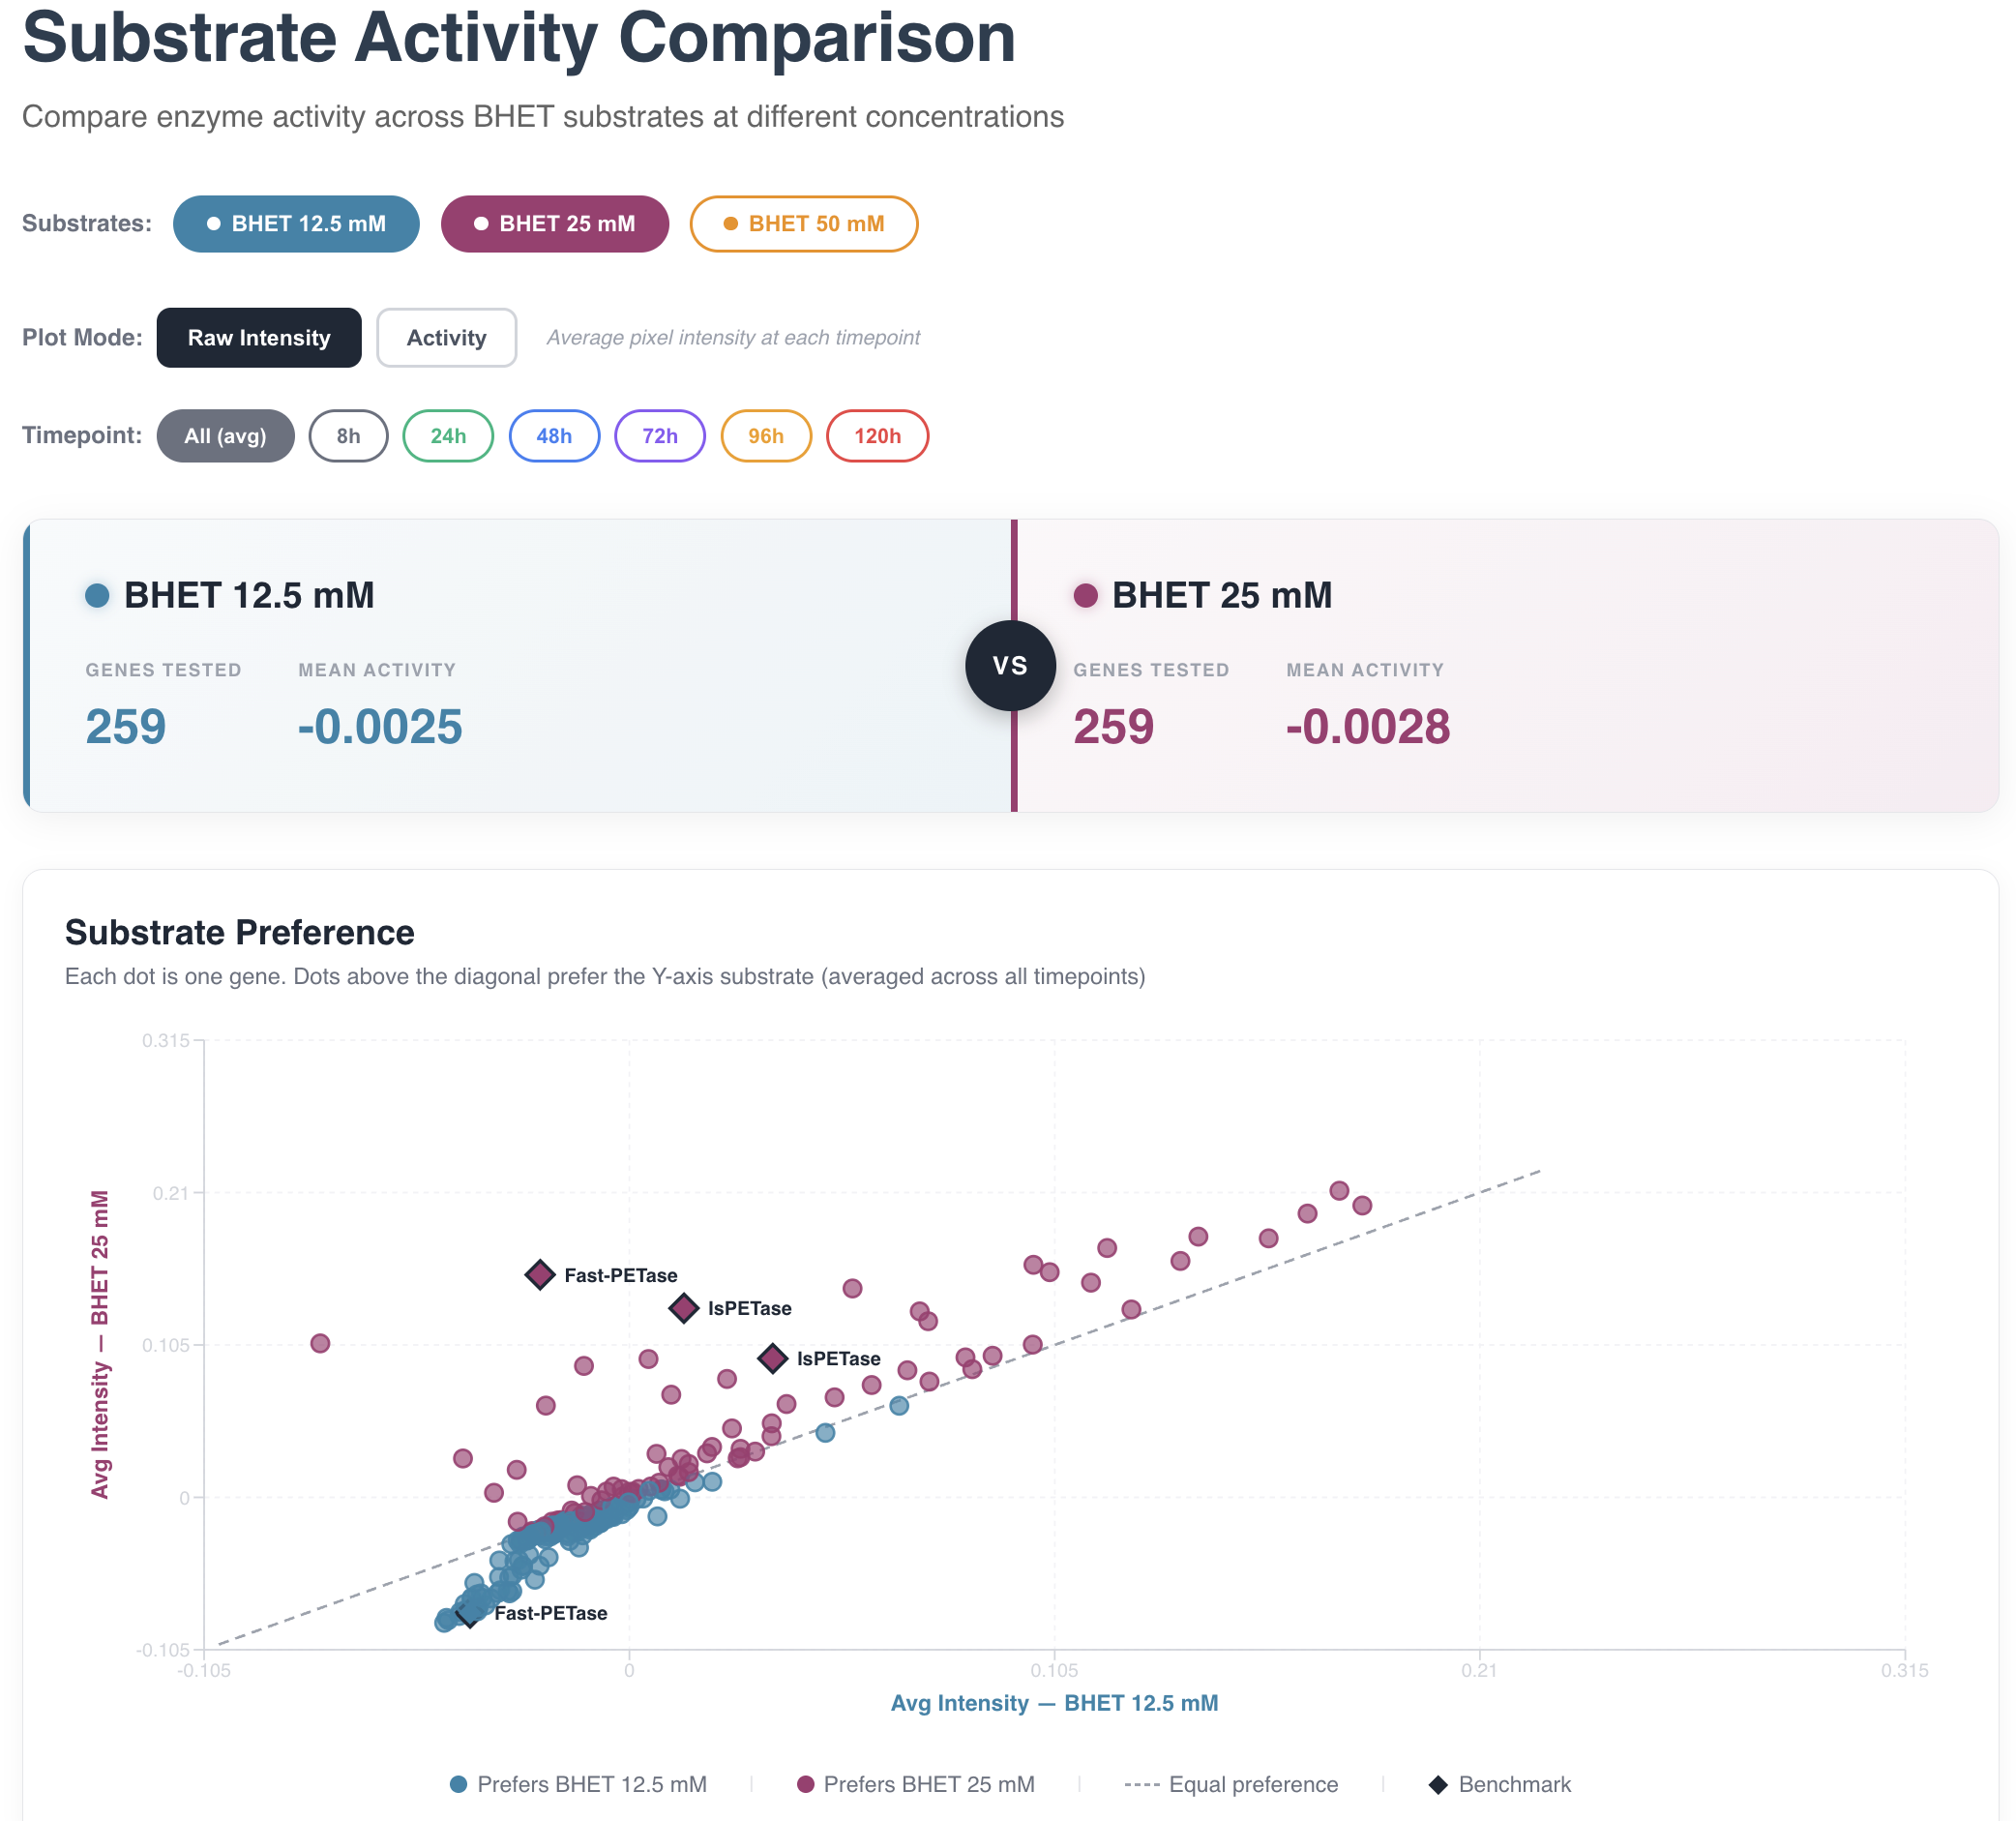
\includegraphics[width=\textwidth]{petadex-substrate.png}
\caption{\textbf{Substrate activity comparison interface.} The substrate page displays BHET hydrolysis data across three concentrations (12.5, 25, and 50 mM) and five timepoints (8, 24, 48, 72, 96 h). \textit{Left:} substrate preference scatter plot in which each point represents one gene, plotted as activity at one BHET concentration versus another; the dashed diagonal marks equal preference. Benchmark enzymes (IsPETase, FAST-PETase) are shown as diamonds. \textit{Right:} representative activity line chart for a single gene showing median pixel intensity over time ($\pm$s.d.) at each substrate concentration, with the computed peak-to-minimum degradation signal indicated.}
\label{fig:substrate}
\end{figure*}

\subsection{Use case: biological signal from the embedding landscape}

The ESM-2 Atlas has proven to be not merely a visualization tool but an instrument for biological discovery. During systematic exploration of the embedding landscape, we identified a set of families that cluster unexpectedly in embedding space despite being assigned to distinct sequence-identity-based families by MMseqs2. Examination of these families revealed that they contain multi-domain architectures in which a PETase-like catalytic domain is fused to one or more additional enzymatic domains, producing so-called ``cocktail enzymes''. Because the sequence-identity clustering operates on full-length sequences, these chimeric proteins are assigned to families that reflect their overall sequence composition rather than their individual domain content. The ESM-2 embeddings, which capture structural and functional features at a deeper level, group these multi-domain proteins together based on shared domain-level similarity, effectively flagging families that may benefit from domain-level decomposition or reclassification.

\begin{figure*}[!htbp]
\centering
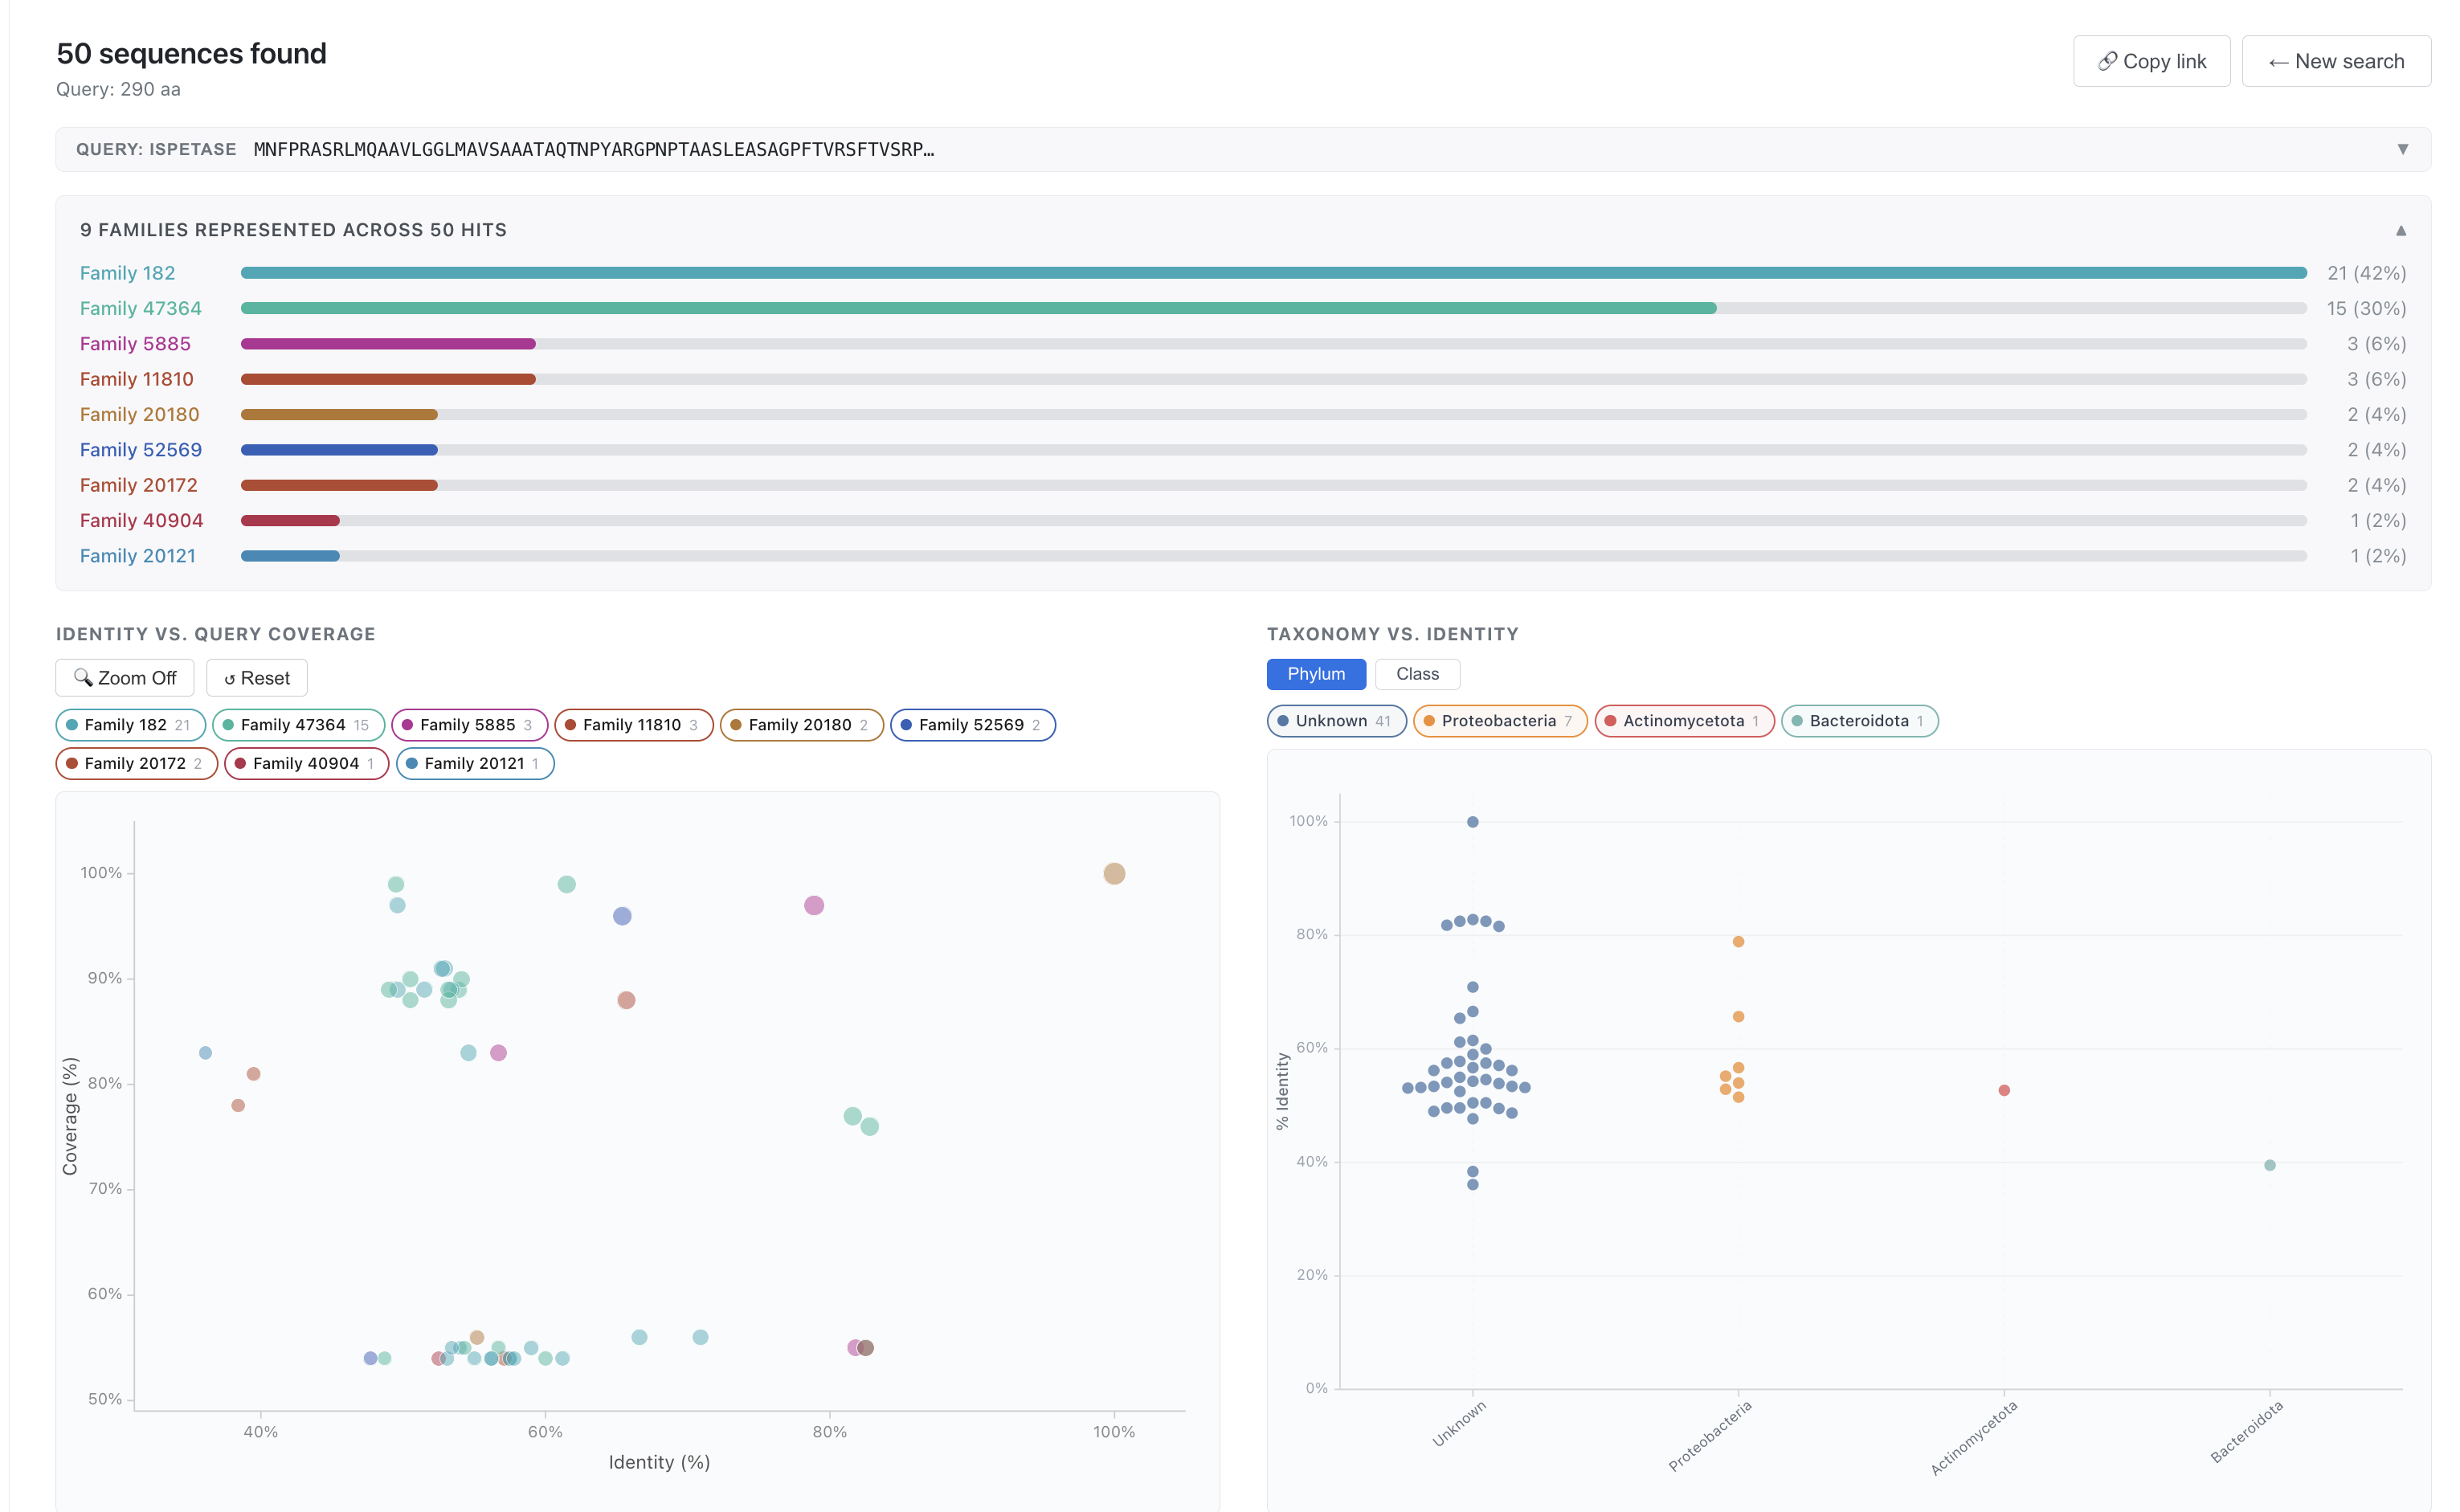
\includegraphics[width=\textwidth]{petadex-figure-4.png}
\caption{\textbf{MMseqs2 search results for IsPETase queried against PETadex.} Beeswarm plot showing the distribution of 50 hits across percent identity, colored by PETadex family assignment. Experimentally characterized enzymes are labeled. The search recovers hits from at least seven distinct families spanning diverse bacterial lineages.}
\label{fig:beeswarm}
\end{figure*}

Cross-referencing the embedding coordinates of these cocktail enzyme families with NCBI environmental metadata revealed a further observation: a subset of these multi-domain families are associated with sequences originating from sulfur-rich, aerobic environments, including volcanic and hydrothermal contexts. The co-occurrence of PETase-like domains in bacteria from sulfur-associated niches raises the possibility of a non-plastic ecological role for these enzymes, or alternatively, convergent recruitment of hydrolase domains in organisms adapted to chemically extreme environments. We emphasize that this association is correlative rather than mechanistic, and the functional significance of these multi-domain architectures in sulfur-rich environments remains to be determined experimentally. Nonetheless, this finding illustrates how PETadex, by combining large-scale sequence data with embedding-based exploration and environmental metadata, can generate testable biological hypotheses that would not emerge from smaller, manually curated datasets.

\subsection{Use case: querying IsPETase against PETadex}

To illustrate the platform's utility for sequence-level exploration, we queried the canonical \textit{Ideonella sakaiensis} PETase (IsPETase, 290 amino acids) against the PETadex database. The search returned 50 hits spanning a wide range of sequence identity, from a perfect self-match (100\% identity, WP\_054022242.1, family 20180) down to remote homologs at 36.1\% identity. The second-ranked hit corresponds to the well-characterized poly(butylene succinate-co-adipate) depolymerase from \textit{Acidovorax delafieldii} (78.9\% identity, family 5885), a known polyester hydrolase and close evolutionary relative of IsPETase. Even within the top 50 results, hits were recovered from diverse bacterial lineages including Betaproteobacteria, Gammaproteobacteria, Actinomycetes, and Bacteroidota, highlighting the broad phylogenetic distribution of PETase-like enzymes beyond the Burkholderiales clade in which IsPETase was originally identified.

The search results mapped to at least seven distinct PETadex families, indicating that PETase-like sequence space is fragmented across multiple evolutionarily distinct enzyme groups rather than forming a single monolithic cluster. Several experimentally validated PET and polyester hydrolases appeared at varying evolutionary distances, including the \textit{Thermobifida cellulosilytica} cutinase (52.7\% identity) and the \textit{Halopseudomonas aestusnigri} hydrolase (51.5\% identity), providing immediate functional context for interpreting the results. A PDB structural entry (7DZT\_A, 82.5\% identity) also appeared among the hits, linking the search directly to available crystallographic data. This example demonstrates how a single sequence query in PETadex can serve as an entry point into the broader landscape of PETase diversity, simultaneously providing family assignments, functional annotations, taxonomic context, and structural cross-references.

%% ============================================================
\section{Discussion}

PETadex represents a fundamentally different kind of resource from existing PETase databases. PAZy, the current gold standard for curated PET-degrading enzymes, catalogues approximately 218 wild-type entries with activity data aggregated from heterogeneous assays across the published literature \citep{buchholz_plastics_2022}. While invaluable for its curation depth, PAZy's activity measurements are drawn from diverse experimental conditions, substrates, and reporting standards, which limits direct quantitative comparison across enzymes. PlasticDB provides a complementary resource linking 329 proteins and 875 species to plastic degradation with associated metadata \citep{gambarini_plasticdb_2022}. Both databases serve as curated literature resources; PETadex, by contrast, is a discovery platform designed to make the full predicted diversity of PET-degrading enzymes from metagenomic data navigable and searchable at a scale of 216.7 million sequences and approximately 65,000 families.

This difference in scope is not merely quantitative. Curated databases, by design, index enzymes that have been individually cloned, expressed, and characterized in the literature, which biases their coverage toward a small number of well-studied enzyme families and culturable organisms. PETadex, by contrast, derives its sequence corpus from an exhaustive search of metagenomic and environmental sequencing data in the SRA, capturing PETase-like diversity from uncultured lineages, undersampled biomes, and taxonomic groups that have never been the focus of directed PET degradation studies. The result is a database that reflects the full predicted sequence landscape of PET hydrolases rather than the subset visible through the lens of traditional enzyme characterization.

A notable advantage of the experimental data within PETadex is its internal consistency. The 259 activity datapoints in the database derive from a single standardized BHET hydrolysis assay performed under uniform conditions, as described in Logan \textit{et al.}\ \citep{chikhi_logan_2025}. This exceeds the number of PET-specific activity entries in PAZy and, critically, enables direct quantitative comparison across enzymes, which data aggregated from heterogeneous literature sources cannot support. The sequence-to-activity join path in PETadex links computational sequence data directly to these standardized measurements, providing a foundation for structure-activity analyses and machine learning applications.

The complementarity between sequence-identity clustering and structure-aware embeddings, as demonstrated by the cocktail enzyme finding in the Atlas, underscores the value of multi-modal data exploration. Sequence-identity-based methods such as MMseqs2 remain the workhorse of large-scale sequence analysis, but protein language model embeddings capture functional and structural relationships that primary sequence similarity alone may miss. By providing both lenses on the same data, PETadex allows researchers to identify patterns that would be invisible from either perspective in isolation.

\subsection{Future directions}

Several extensions of PETadex are planned or underway. First, we are developing automated pipelines to scrape, normalize, and integrate published activity data from PAZy, the primary literature, and supplementary tables, which will substantially expand the experimentally grounded fraction of the database and enable more comprehensive structure-activity mapping. Second, PETai, a machine learning pipeline that uses ESM-2 embeddings and graph neural networks to predict PETase activity from sequence and structural features, is being developed using PETadex as its training foundation. Third, we plan to extend structural annotation at scale, leveraging AlphaFold2 \citep{jumper_highly_2021} and ESMFold \citep{lin_evolutionary-scale_2023} predicted structures for family centroids. Longer-term goals include community submission tools that would allow researchers to deposit new sequences and activity measurements, and integration with iGEM synthetic biology workflows to support educational and engineering applications.

%% ============================================================
\section{Data Availability}

PETadex is freely available at \url{https://petadex.net}. The database can be queried through the web interface or programmatically via the REST API. Source code for the web platform is available at [GitHub URL]. The underlying sequence data and clustering are described in Logan \textit{et al.}\ \citep{chikhi_logan_2025}.

%% ============================================================
\section{Acknowledgements}

D.Z.\ developed the PETadex web platform, database architecture, serverless backend, sequence search infrastructure, ESM-2 embedding landscape, data visualizations, and NCBI metadata enrichment pipeline. The petaSearch sequence discovery pipeline and BHET activity assay data were generated by Logan \textit{et al.}\ \citep{chikhi_logan_2025} under the supervision of A.B. InterProScan annotations were computed on the Donnelly Centre computing cluster. We thank the members of the Babaian laboratory and iGEM Toronto 2026 for valuable discussions.

%% ============================================================
\section{Funding}

[Funding information to be added.]

%% ============================================================
\bibliographystyle{oup-abbrvnat}
\bibliography{petadex-references}

\end{document}